実験1では, 認証機構が正しく機能していることを確認するための実験を
行った. 不正ノードが存在する環境で, パケット配送率(PDR)とスループットを測定し, 
EdDSAによってセキュリティがどの程度確保されているのかを評価した. 
適度に影響が出るよう, 第2章で述べた2種類の不正ノードを, 送信ノードの近辺, 送受信ノードの
中間, それ以外の位置に1個ずつ用意し, 
全ノードの約8\% (計6個)を不正ノードに設定した. また, 結果のばらつきを
抑えつつ, 統計的な評価を行うために, 250回シミュレーションを行い, 
パケット配送率 (PDR)とスループットを調べた. 
実験1の主なシミレーションパラメータは表\ref{tab:exp1-params}に示す通りである.
\begin{longtable}{cc}
  \caption{実験1のシミュレーションパラメータ}
  \label{tab:exp1-params}
  \endfirsthead
  \hline
  シミュレーション時間 & 300[s] \\
  ノード数 & 74 \\
  送受信ノードのペア数 & 1 \\ 
  不正ノード & あり \\ \hline
\end{longtable}
\vspace{1em}
\indent 実験結果を図\ref{fig:exp1_pdr}, 図\ref{fig:exp1_throughput}に示す. \\[-2.5em]
\begin{figure}
  \centering
  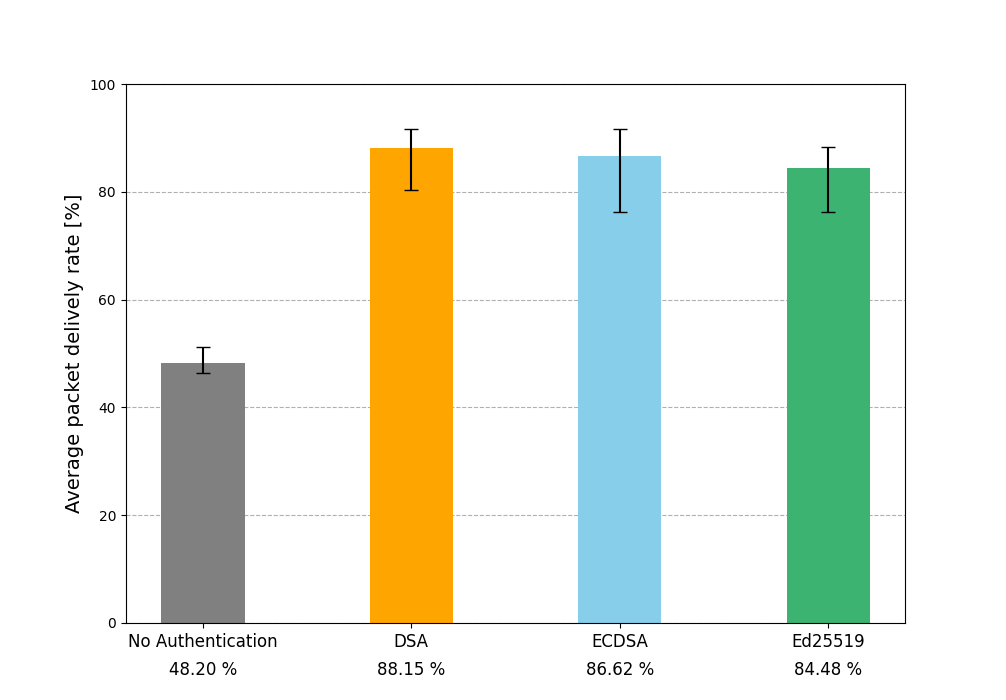
\includegraphics[width=1\textwidth]{figures/exp1_pdr.png}
  \caption{不正ノードが存在する環境でのパケット配送率}
  \label{fig:exp1_pdr}
\end{figure}
\clearpage
\begin{figure}
  \centering
  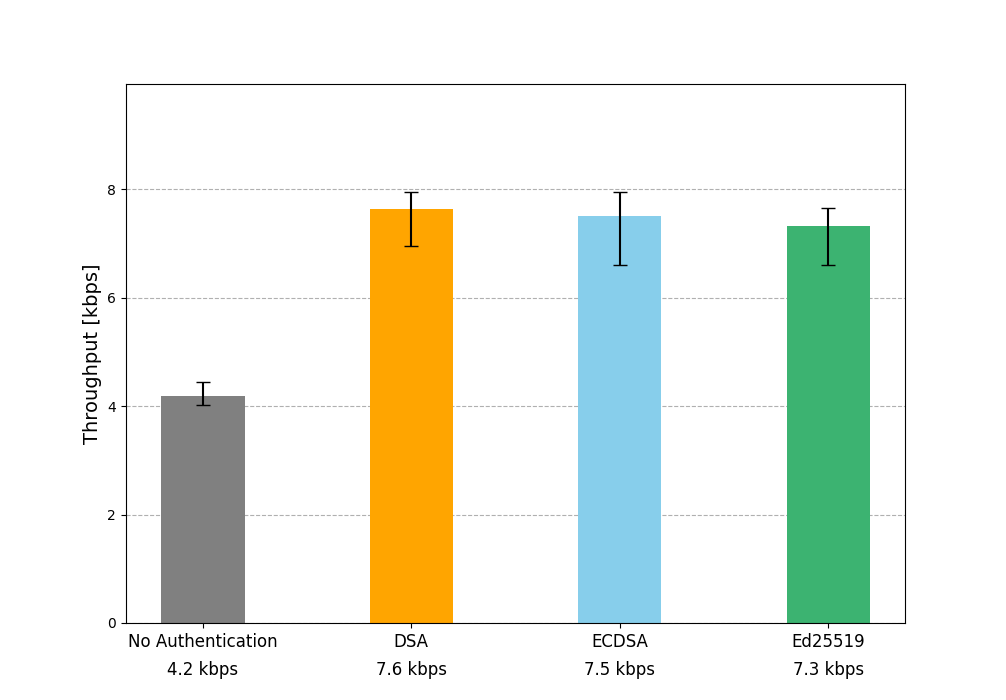
\includegraphics[width=1\textwidth]{figures/exp1_throughput.png}
  \caption{不正ノードが存在する環境でのスループット}
  \label{fig:exp1_throughput}
\end{figure}


\indent 図\ref{fig:exp1_pdr}は, 実験1におけるシミュレーションパターンごとの
パケット配送率を示している. 認証機構なしの場合に48.2 \%であるのに対し, 
ECDSAでは86.62 \%, EdDSAでは84.48 \%と, 認証機構を追加したことでパケット配送率が
約30 \%向上した. \\
\indent 図\ref{fig:exp1_throughput}は, 実験1におけるシミュレーションパターンごとの
スループットを示している. 認証機構なしの場合に4.18kbpsであるのに対し, 
ECDSAでは7.51kbps, EdDSAでは7.33kbpsと, 認証機構を
追加することでパケット配送率同様, スループットも向上した. \\
\indent これらの結果は, 認証機構の追加により 
不正ノードが排除されたことで, 経路選択を行う際に正当なノードのみが
選択されており,  データの窃取(転送中止)が回避できたことを示している. 
また, EdDSAの結果をECDSAの結果と比較するとほとんど差がないため, 
2つの署名方式が不正ノードを排除することにおいて同等のセキュリティ性能をもつと考えられる. 



